\documentclass[conference]{IEEEtran}
\IEEEoverridecommandlockouts
% The preceding line is only needed to identify funding in the first footnote. If that is unneeded, please comment it out.
\usepackage{cite}
\usepackage{amsmath,amssymb,amsfonts}
\usepackage{algorithmic}
\usepackage{graphicx}
\usepackage{textcomp}
\usepackage{xcolor}
\usepackage[backend=bibtex]{biblatex}
\addbibresource{References.bib}

\usepackage{listings}
\usepackage{xcolor}
\usepackage{caption}
\usepackage{booktabs}
\lstset{
  basicstyle=\ttfamily\footnotesize,
  backgroundcolor=\color{gray!10},
  frame=single,
  breaklines=true
}

\usepackage{tabularx}
\usepackage{adjustbox}


\def\BibTeX{{\rm B\kern-.05em{\sc i\kern-.025em b}\kern-.08em
    T\kern-.1667em\lower.7ex\hbox{E}\kern-.125emX}}
\begin{document}

\title{ Dynamic Sporadic Server\\

}

\author{\IEEEauthorblockN{ Moiz Zaheer Malik}
\IEEEauthorblockA{\textit{ B.Eng. Electronic Engineering} \\
\textit{Hochschule Hamm-Lippstadt}\\
Lippstadt, Germany \\
moiz-zaheer.malik@stud.hshl.de}

}

\maketitle

\begin{abstract}
In real-time systems, where tasks have different levels of critical importance, it is essential to serve aperiodic (irregular, event-driven) tasks while ensuring that the deadlines of high-priority periodic tasks are not violated. The Dynamic Sporadic Server (DSS) is a scheduling method designed for Earliest Deadline First (EDF) systems that addresses this problem. 

DSS is defined by a period  $T_s$ and a budget $C_s$, but unlike traditional sporadic servers, it does not restore the full budget at every period. Instead, when an aperiodic task arrives, DSS assigns it a deadline and restores only the amount of budget that was actually used. This approach allows the processor to reach full (100 percent) utilization while ensuring that all deadlines are still met. DSS improves the response time of aperiodic tasks without compromising the guarantees of periodic tasks.

Originally introduced by Spuri and Buttazzo\cite{spuri1994efficient}, DSS has been widely studied for its efficiency in managing mixed task sets under EDF scheduling. This report reviews the theory behind DSS, describes its operation (including budget management), highlights its advantages over traditional methods, and discusses potential application areas.
 
\end{abstract}

\section{Introduction}

Real time system often mix periodic tasks (reccurring tasks with fixed periods and deadlines) and aperiodic/sporadic tasks (tasks which arrive unpredictavly), for example interrupts or user request) And to ensure that the aperiodic tasks recive their service on time without causing problem to any aperiodic tasks to miss their deadlines is a majr challeng\cite{laplante2011real}. 

A common solution is to use Server Abstraction it is a concept used in real time systems to mannage how and when tasks (especially aperiodic or sporadic) are executed. Such as Polling Server, Deferrable server, and sporadic servers. The sporadic servers, introduced by Sprunt et al\cite{sprunt1989aperiodic}, assigns a fixed priorarity (typically through Tate Monotonic) to the server and provides a budget $C_s$ every period $T_s$. This allows aperiodic tasks to be executed with limited interference to hard real time tasks. However, under staticprority scheduling the processor often cannot be fully utilized, unused server budget might be wasted or caused complex analysis.

with dynamic scheduling (EDF) higher utilization can be achived. Dynamic priority server as shifted the sporadic server concept to (EDF). In particular, spuri and Buttazzo proposed the Dynamic Sporadic Server (DSS)\cite{spuri1994efficient}. Dss is characterized by a server period $T_s$ and capacity $C_s$ (the maximum aperiodic budget)\cite{buttazzo2011hard}. Unlike SS, DSS does not refill or replenish $C_s$ fully at each period start. Insted, the server's deadline and replenishment events are set dynamiclly whenever aperiodic work arrives or is consumed\cite{spuri1994efficient}. This allowes DSS to adaptivly use idle time for aperiodic tasks and to achive 100 percent CPU utilization. 

But the most important requirment is that under EDF schedule, the sum of the utilization of periodic tasks ($U_p$)\cite{buttazzo2011hard} plus the utilization of DSS ($U_s = C_s/T_s$)\cite{buttazzo2011hard} must satisfy In order to meet all deadlines\cite{spuri1994efficient}. 

\[
U_p + U_s \leq 1
   \ \cite{buttazzo2011hard} \]
   
Just like EDDF alone, DSS with EDF still allows 00 percent Cpu usage, so periodic tasks dont lose processing time. Unlike EDF, a fixed priority sporadic server cant fully use the CPU unless more complex analysis is done\cite{spuri1994efficient}.
   
\section{BACKGROUND: PERIODIC AND APERIODIC TASKS; EDF}
\textbf{Periodic task:} A periodic task $\tau_i$ generates tasks again and again, each job needs exeution time $C_i$ and must finish by a deadline $D_i$ after its arrival. commonly, $D_i = T_i$ (Deadline is equal to Period). The total Utilization of the periodic task is 

\[
U_p = \sum_i \left( \frac{C_i}{T_i} \right)
\ \cite{buttazzo2011hard} \]

based on the study by Liu and Layland\cite{liu1973scheduling}, The EDF algorithm can successfully schedule any set of periodic task (where deadlines are equal to periods) if and only if 

\[
U_p \leq 1
\ \cite{buttazzo2011hard} \]

\textbf{Aperiodic tasks:} More genral then sporadic, aperiodic tasks include all kind of arrivals, even the ones not allowed under sporadic rules. Aperiodic tasks can be unpridictable, they ussally have soft deadlines, which means they can somtimes miss ther deadlines. To measure how much CPU they need, we can look at their average or maximum load $U_a$. And the main goal of it is to serve these tasks quickly without effecting periodic tasks that have strict dedlines\cite{buttazzo2011hard}

\textbf{sporadic task:} Is a task comes at random times but with a rule there must be minimum gap (period)$T_s$ between two jobs. each job needs some time to run and execut $C_s$. Even though the job arive at irregularly, this minnimum gap helps to keep things under control. Because of this sporadic tasks are seen as simpler kind of periodic tasks with more flexible timing.\cite{buttazzo2011hard}.

\textbf{EDF Scheduling:}  Under EDF, tasks are assigned dynamic priorities equal to their absalut deadline (Earliest dealine = Highest ppriority). The EDF schedulability criterion rule workes with both periodic and aperodic tasks but only when tasks are treated like sporadic tasks with deadlines\cite{spuri1994efficient, buttazzo2011hard}.

However, simpl qeueing all periodic tasks under EDF can still cause problems for periodic tasks. Therefore server algorithms are used to controle how much CPU the aperiodic workload can use, effectively reserving bandwidth for aperiodic server\cite{buttazzo2011hard}. DSS is one such server, whch is used in EDF based system\cite{buttazzo2011hard}.

\section{SPORADIC AND DYNAMIC SERVERS}
\subsection{The Sporadic Server (SS)} 

Before DSS, Sporadic server (SS) was used initially for fixed priority scheduling\cite{buttazzo2011hard}. The parameters of sporadic server are ($T_s$,$C_s$), Its rule is When an aperiodic task arrives and the serevr has avilable capacity, the server executes that job at high priority as long as it has budget. after consuming a amount of execution $U$, the server schedules a refil of $U$ after one period $T_S$\cite{buttazzo2011hard}.. The SS makes sure that the server uses as much of the the $C_s$ time in a period od $T_s$, ensuring pariodic tasks guarantees only if\cite{buttazzo2011hard}

\[
U_p + \frac{C_s}{T_s} \leq 1
\ \cite{buttazzo2011hard} \]

Where $U_p$ is the utilization of periodic taasks. However, in SS the serverperiority is fixed, making it not directly suitable for EDF system\cite{buttazzo2011hard}.

\subsection{The Dynamic Sporadic Server (DSS)}
The Dynamic Sporadic server (DSS) modifies the sporadic server (SS) for EDF Scheduling\cite{spuri1994efficient}.
Like SS, DSS has a server period $T_s$ and a Capacity $C_s$, DSS has dynamic deadlines rather than a fixed priority. the server the server behaves like EDF task whose deadline is recalculated at runtime when ever it begins servicing an aperiodic task. it budget does not resets simply at $T_s$, insted it's only consumed portions are recharged after $T_s$ units\cite{spuri1994efficient,buttazzo2011hard}.

The DSS behaves in the following way,
\textbf{Initialization:} The server starts with full budget $C_s$. No deadline $d_s$ is set until the first aperiodic job arives\cite{spuri1994efficient,buttazzo2011hard}.

\textbf{Activation:} When an aperiodic task arrives aat time $t_A$ and the server is idle with available budget $>0$, the server sets its current deadline $d_s$ = $t_A$ + $T_s$\cite{spuri1994efficient} and schedules its next refil at $R_T$ = $d_s$\cite{spuri1994efficient}. The server immediatly becomes the heighest priority EDF task and begins executing aperiodic ask. All aperiodic taskin that busy interval share the same deadline $d_s$\cite{spuri1994efficient}.

\textbf{Execution:} The server executes, deducting from its remaining capacity as it runs aperiodic tasks. If the aperiodic workload finishes before the udget is exhausted, the server waits with leftover budget. If more tasks arrive while budget remain, they are queued but served under the same deadline\cite{spuri1994efficient}. 

\textbf{Budget Exhaustion or Job Completion:} When capacity is exhausted or the last pending task finishes at time $t_I$, the server computes how much budget $u$ was consumed since $t_A$ and schedules a refil of amount $u$ at time $R_t$. if pending tasks remain after exhaustion, they are paused until the refil\cite{sprunt1989aperiodic, spuri1994efficient} 

\textbf{Next Activation:} afetr refil at every $R_T$, if there are tasks pending the server repeates the activation step, it sets a new deadline $d_s$ = $R_T$ + $T_s$ and executes again. 

These rules ensure ever consumes more the the $C_s$ time in any period $T_s$\cite{spuri1994efficient,buttazzo2011hard}. Thus DSS behaves like aperiodic task under EDF. The schhedulability condition for mixing DSS with periodic task is\cite{buttazzo2011hard}
\[
U_p + U_s = \sum_i \frac{C_i}{T_i} + \frac{C_s}{T_s} \leq 1
\ \cite{buttazzo2011hard, spuri1994efficient} \]

Where $U_p$ is the utilization of periodic task and $U_s$ = $C_s$/$T_s$ is servers utilization\cite{buttazzo2011hard}.

\textbf{Mathematical Formulation:} Formally, it can be shown (Lemma and Theorem in~\cite{spuri1994efficient}) that in any busy interval of length $\Delta$, the server executes at most $C_s$ time per $T_s$ window. 
Thus, DSS achieves full utilization in EDF-based systems, as long as $U_p + U_s \leq 1$  \cite{buttazzo2011hard}.

\section{Dynamic Sporadic Server Simulation}
\begin{figure}
    \centering
    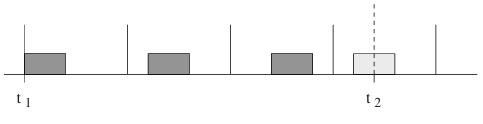
\includegraphics[width=1\linewidth]{image.png}
    \caption{Dynamic Sporadic Server example\cite{buttazzo2011hard}}
    \label{fig:enter-label}
\end{figure}

In this example, we simulate two periodic tasks τ1 and
τ2 along with a Dynamic Sporadic Server (DSS) that serves
incoming aperiodic requests. Task τ1 has period P1 = 8
and execution time C1 = 2, while τ2 has P2 = 12 and
C2 = 3. The DSS is configured with period Ts = 6 and
capacity Cs = 3. Aperiodic tasks arrive at specific times (for
example at t = 3, 6, 9, . . . with varying execution demands)
and are queued for service by the DSS. The scheduler uses
earliest-deadline-first (EDF) policy, breaking ties in favor of
the server[2, 8].
The DSS logic follows the standard rules: its budget is
initialized to Cs and is replenished one period after each
activation[8]. Whenever a new aperiodic request arrives and
the server is idle with remaining budget, the server becomes
active, and its deadline is set to (current time + Ts)[8]. While
active, the server executes as long as there is pending aperiodic
work and budget remains; each execution unit decrements
both the server’s remaining capacity and the active aperiodic
job’s remaining work. If the server exhausts its budget or
completes all queued aperiodic tasks, it becomes inactive
and schedules its consumed budget to be replenished at the
previously assigned deadline\cite{buttazzo2011hard}

\section{DSS-Based UPPAAL Model Simulation}
\begin{figure}
    \centering
    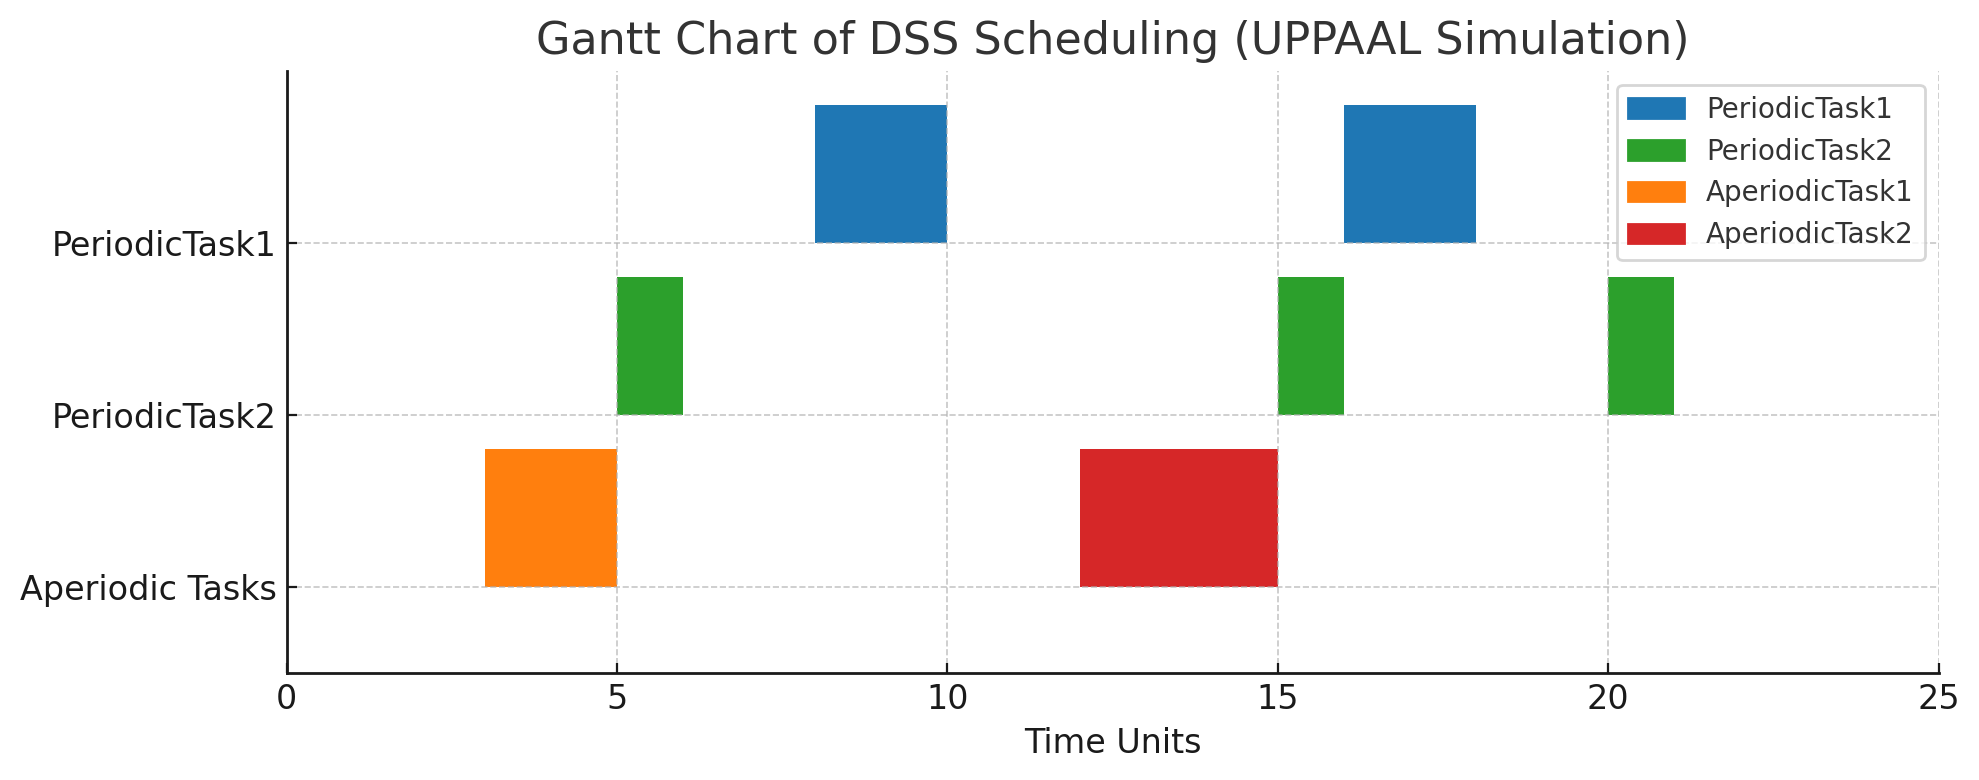
\includegraphics[width=1\linewidth]{06aa5266-f51e-41c8-a4c3-ac8c8555d283.png}
    \caption{Gantt chart}
    \label{fig:enter-label}
\end{figure}
\begin{figure}
    \centering
    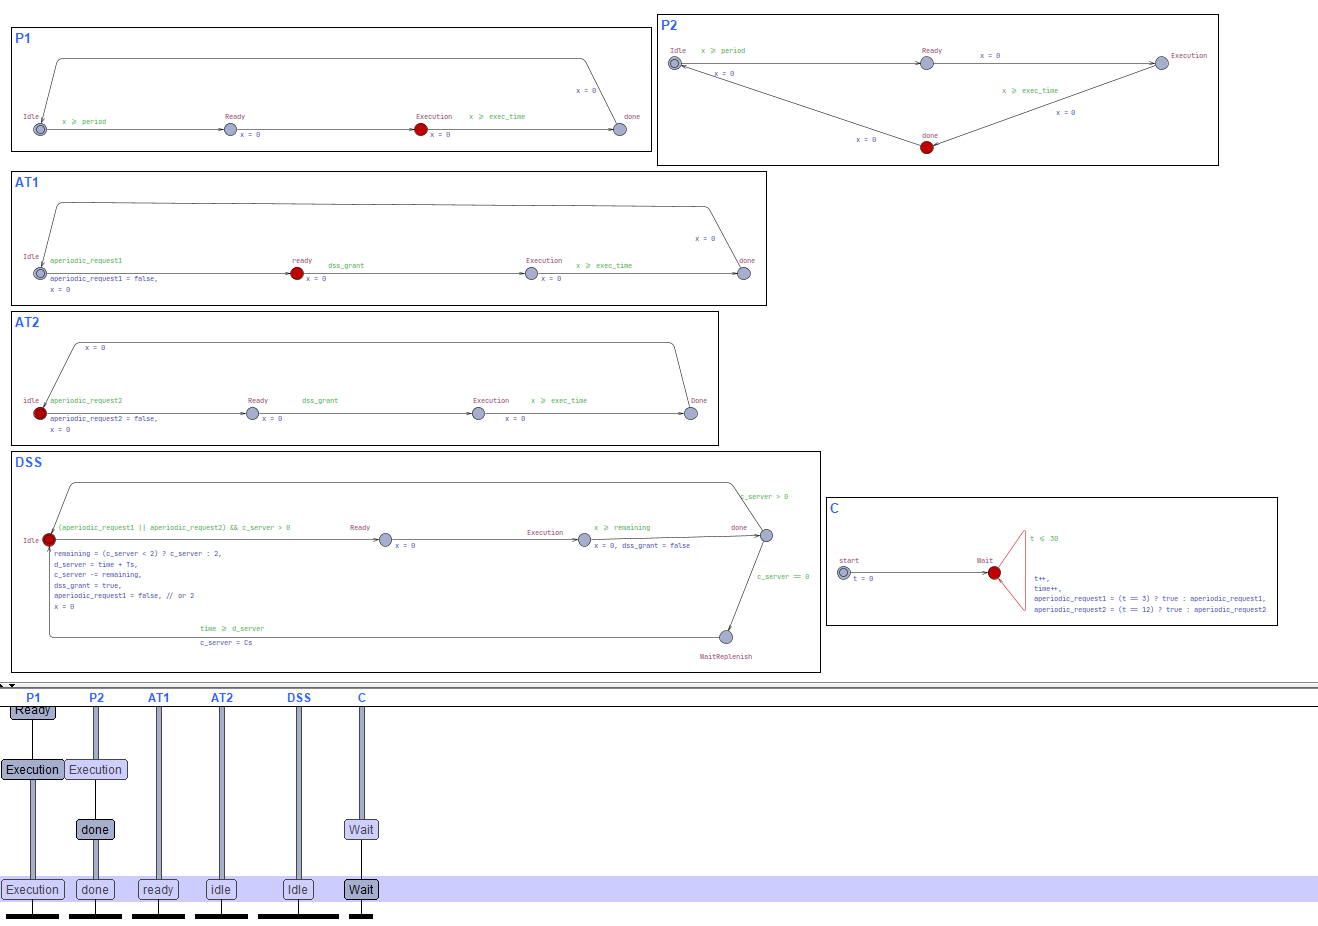
\includegraphics[width=1\linewidth]{Screenshot 2025-05-31 210123.png}
    \caption{Symbolic Simulator}
    \label{fig:enter-label}
\end{figure}
\begin{figure}
    \centering
    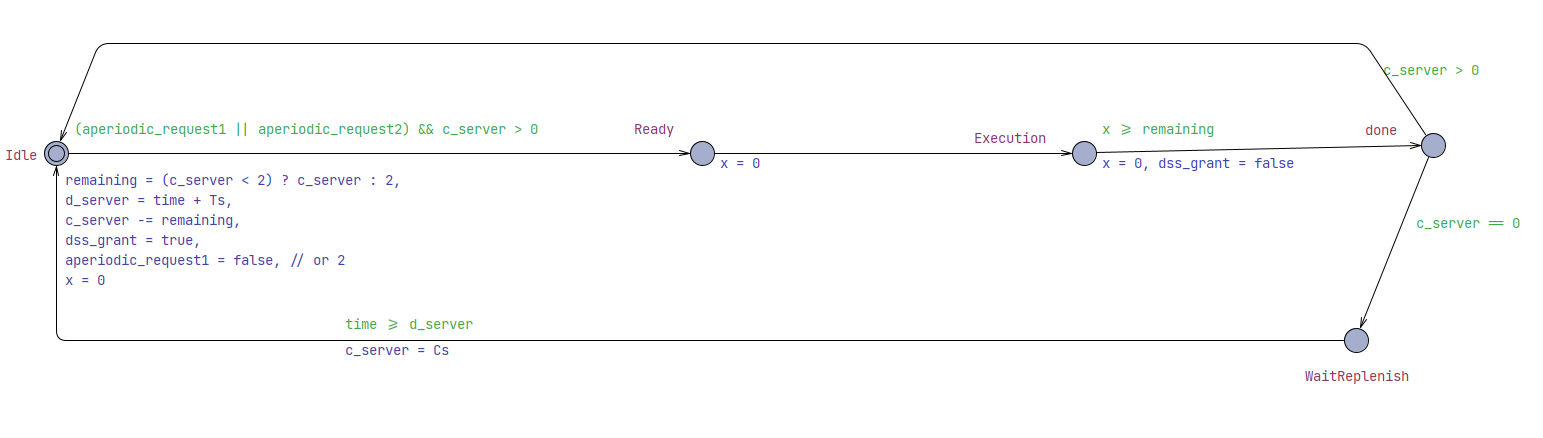
\includegraphics[width=1\linewidth]{DSS Server.png}
    \caption{DSS server}
    \end{figure}
\begin{figure}
    \centering
    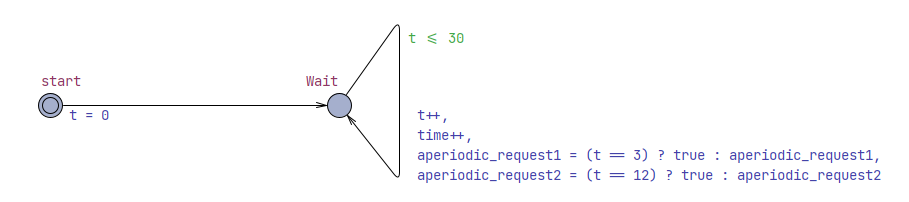
\includegraphics[width=1\linewidth]{Controller.png}
    \caption{Controller}
        \label{fig:enter-label}
\end{figure}
 \begin{figure}
        \centering
        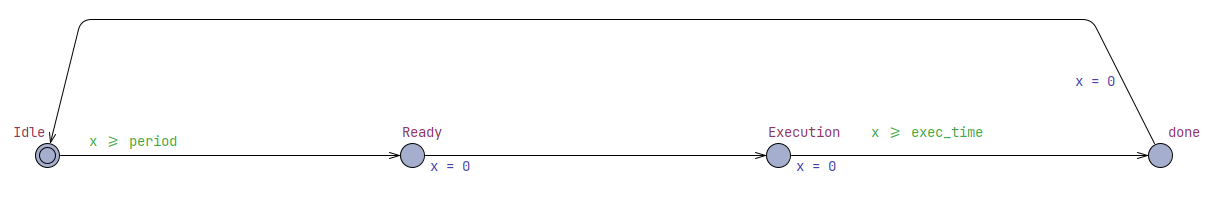
\includegraphics[width=1\linewidth]{PT1.png}
        \caption{Periodic Task 1}
         \label{fig:enter-label}
    \end{figure}
\begin{figure}
            \centering
            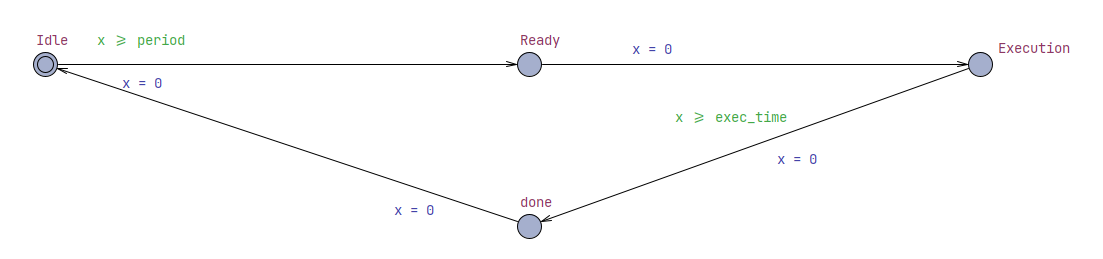
\includegraphics[width=1\linewidth]{PT2.png}
            \caption{Periodic Task 2}
             \label{fig:enter-label}
        \end{figure}
\begin{figure}
                \centering
                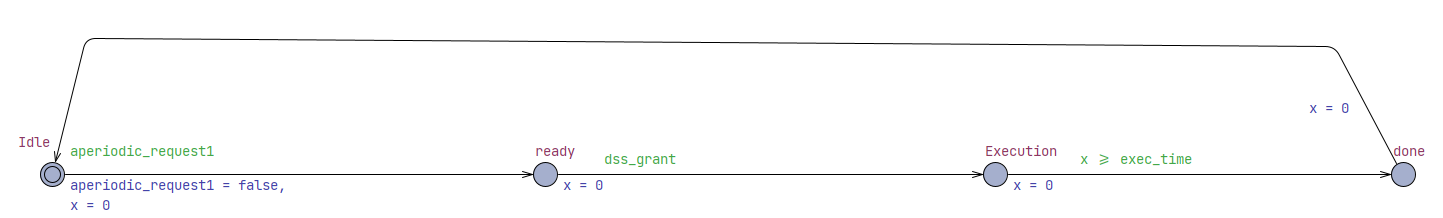
\includegraphics[width=0.75\linewidth]{APT1.png}
                \caption{Aperiodic Task 1}
                \label{fig:enter-label}
            \end{figure}
            \begin{figure}
    \centering
    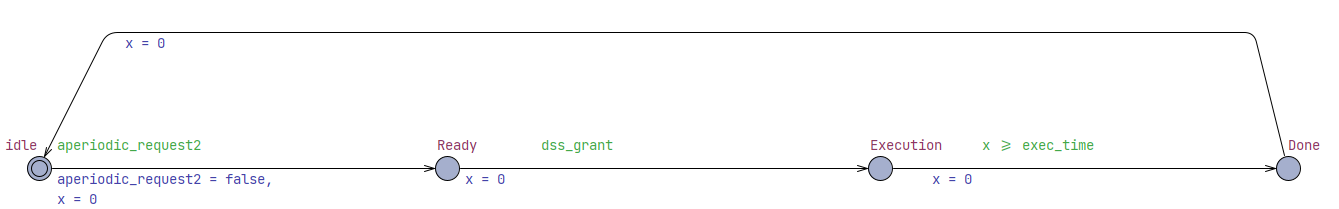
\includegraphics[width=0.75\linewidth]{APT2.png}
    \caption{Aperiodic Task 2}
    \label{fig:enter-label}
\end{figure}
In this seminar, I presented a simulation of the Dynamic Sporadic Server (DSS) model using the UPPAAL tool. The main aim was to show how DSS scheduling can handle aperiodic tasks without interfering with periodic tasks, which is very important in real-time systems. The simulation I made includes two periodic tasks, two aperiodic tasks, a DSS server, and a controller that acts as the environment.

The periodic tasks are designed to run at fixed intervals. \textbf{PeriodicTask1} has a period of 8 time units and executes for 2 time units, while \textbf{PeriodicTask2} has a shorter period of 5 units and executes for 1 time unit. Each periodic task moves through four states: \textit{Idle}, \textit{Ready}, \textit{Execution}, and \textit{Done}. When the period expires, the task moves to \textit{Ready}, then executes for its set time, and then goes to \textit{Done} before resetting.


For the aperiodic part, I included two tasks that are not triggered by time but by events. \textbf{AperiodicTask1} runs for 2 units and is triggered by the controller at time $t = 3$. \textbf{AperiodicTask2} runs for 3 units and is triggered at $t = 12$. However, these tasks can’t just start on their own. They must be allowed by the DSS server through a signal called \texttt{dss\_grant}. This means that even if a request comes in, the task will only run if the DSS says it can.

The \textbf{DSS\_Server} is the key part of the whole model. It manages when and how aperiodic tasks can execute. The server has a capacity ($C_s$) of 3 units, which means it can spend up to 3 time units on aperiodic tasks before it needs to refill. The replenishment period ($T_s$) is 6 units, so every 6 units, it gets its full capacity back. The DSS goes through several states: \textit{Idle} (watching for new requests), \textit{Ready} (when it decides to grant access), \textit{Execution} (running an aperiodic task), \textit{Done} (after the task finishes), and \textit{WaitReplenish} (when it has no capacity and is waiting to refill). It keeps track of how much capacity it has left using the variable \texttt{c\_server} and also remembers when to refill with \texttt{d\_server}.

The \textbf{Controller} in the model is a simple component that simulates the environment. It keeps track of time and triggers the aperiodic task requests at specific points. In my simulation, it sets \texttt{aperiodic\_request1 = true} at $t = 3$ and \texttt{aperiodic\_request2 = true} at $t = 12$. It also increases logical time step by step.

When the simulation runs, both periodic tasks start in \textit{Idle}. At time $t = 3$, the controller triggers the first aperiodic request. Since DSS has full capacity at the start, it grants permission, and \textbf{AperiodicTask1} executes. This reduces the server's capacity by 2 units. Then, periodic tasks keep executing according to their periods \textbf{PeriodicTask2} runs at $t = 5$ and \textbf{PeriodicTask1} at $t = 8$. At $t = 12$, the controller sends the second aperiodic request. Now, depending on how much capacity the DSS has left, it may either run the task or wait until its capacity is replenished.

The simulation clearly shows how DSS works to let aperiodic tasks execute without breaking the schedule of the periodic ones. The DSS carefully tracks how much capacity is used and refills only after the defined period. This method ensures that periodic tasks always get priority and deadlines are not missed, while still giving space to aperiodic tasks when possible. I believe this model demonstrates the concept in a simple but effective way, and helps to understand real-time scheduling more practically.

\section{Comparison with Other Servers}
Table~\ref{tab:servers} compares key features of Polling, Deferrable, Sporadic, and Dynamic Sporadic servers.  Polling servers operate under fixed-priority scheduling and reset their budget at each period regardless of use \cite{sprunt1989aperiodic}.  Deferrable servers also run at high priority but carry unused capacity to the end of the period \cite{buttazzo2011hard}.  The classic Sporadic Server (for Rate-Monotonic scheduling) replenishes only the portion of its budget that was actually consumed \cite{sprunt1989aperiodic}.  


\begin{table}[ht]
\centering
\renewcommand{\arraystretch}{1.1} % Optional: add some vertical spacing
\begin{tabularx}{\columnwidth}{l|X|X|X|X}
\textbf{Feature} & \textbf{Polling} & \textbf{Deferrable} & \textbf{Sporadic} & \textbf{DSS} \\
\hline
Scheduling & Fixed-priority (RM) & Fixed-priority (RM) & Fixed-priority (RM) & Dynamic (EDF) \\\\
Priority & Highest static & Highest static & Static (RM) & Dynamic (deadline $t+T_s$) \\\\
Replenishment & Periodic full & Periodic full & On-demand & On-demand \\\\
Unused Budget & Lost if unused & Carried to period end & Carried to next period & Reused flexibly \\\\
Utilization & Often suboptimal & Improved response & Moderate & Full (up to 100\%) \\\\
\end{tabularx}
\caption{Comparison of Aperiodic Servers}
\label{tab:servers}
\end{table}


DSS stands apart by its EDF-based policy and flexible budget usage.  In practice, DSS provides the responsiveness of a high-priority server without leaving CPU time idle when aperiodic demand is present \cite{buttazzo2011hard, laplante2011real}.

\section{Applications and Use Cases}

\printbibliography


\vspace{12pt}
\color{red}


\end{document}
